\documentclass[10pt]{article}
\usepackage[T1]{fontenc}
\usepackage{helvet}
\renewcommand{\familydefault}{\sfdefault}
\usepackage[a4paper,margin=0.65in]{geometry}
\usepackage{graphicx}
\usepackage{xcolor}
\usepackage{amsmath}
\usepackage{booktabs}
\usepackage{enumitem}
\usepackage{placeins}
\usepackage[font={sf,footnotesize},labelfont={sf,bf,footnotesize},justification=justified,singlelinecheck=false]{caption}
\usepackage{hyperref}
\hypersetup{colorlinks=true,linkcolor=blue!50!black,urlcolor=blue!50!black}
\setlength{\parskip}{0.5em}
\setlength{\parindent}{0pt}
\setlist{itemsep=0.2em,topsep=0.2em}
\newcommand{\um}{\,$\mu$m}
\newcommand{\figref}[1]{Fig.~\ref{fig:#1}}

\title{Mesoscope vs BWM: supervised decoding of task variables}
\author{Michael Schartner, Samuel Picard, International Brain Laboratory, Claude Opus 5.5}
\date{IBL mesoscope pilot analysis, v7, \today}

\begin{document}
\maketitle

\begin{abstract}
\noindent The clearest result concerns wheel speed. From 20 random neurons per bin, the mesoscope decodes wheel speed far worse than superficial BWM units ($R^2$ 0.05 vs 0.25; \figref{decoding_n20}), yet the signal is not missing. Only about 3.5\% of mesoscope neurons track wheel speed replicably, against 22\% of BWM units at every recording depth (Figs.~\ref{fig:depth}, \ref{fig:population}), and the best 10 neurons of a mesoscope session predict held-out wheel speed as well as the best 10 BWM units ($r$ 0.50 vs 0.47; Figs.~\ref{fig:rasters}, \ref{fig:population}). The gap therefore reflects how sparse wheel neurons are in the imaged population, not imaging depth, calcium lag or the decoder, which passed every check (\figref{checks}); most of any wheel $R^2$ is the stereotyped speed profile after movement onset. Conversely, the mesoscope has about twice the fraction of stimulus-side-tuned neurons of superficial BWM (15\% vs 7.5\%; \figref{tuning}; part of it one mouse's SSp-ul hotspot), and with 20 neurons it decodes stimulus side and feedback as well as superficial BWM, while choice stays weaker. Bin by bin, the maps of the two modalities correlate positively but not significantly once spatial smoothness is accounted for, with only 25 shared bins (\figref{summary}). Quality control along the way found wheel-encoder overflow in 16 mesoscope sessions (fixed) and task--imaging clock offsets in 2 (excluded).
\end{abstract}

The same task variables are mapped across dorsal cortex for two-photon mesoscope imaging and Neuropixels recordings. Each isocortex neuron is placed in one ML--AP hexagonal bin, 1\,mm across, and both modalities go through identical tests and decoders (the analysis windows differ, see below). BWM is shown twice: units within 640\um{} of the pial surface, the main comparison, and units at all depths.

\section*{What changed in v7 (15 Oct)}
The wheel-speed decoding was checked from the ground up, and the maps were redone:
\begin{itemize}
  \item \textbf{1\,mm hexagons} are the default.
  \item \textbf{Deeper BWM voxels.} BWM units within 640\um{} of the pial surface are the main comparison: twice the mesoscope imaging depth (174--318\um), so ephys units the mesoscope may still see are included generously. This keeps 2{,}929 of 13{,}002 units.
  \item \textbf{A revised wheel decoder.}
  \item \textbf{20 random neurons per bin}, mean over 10 draws.
\end{itemize}
Main findings:
\begin{itemize}
  \item \textbf{A bug in the mesoscope wheel data.} 16 of 153 sessions had wheel-encoder overflow jumps ($\pm$6.6 million rad), so their earlier wheel $R^2$ was meaningless. They are fixed now; no BWM session was affected.
  \item \textbf{Two mesoscope sessions excluded.} Their task and imaging clocks are offset by 146 and 338\,s, so every variable decoded at chance; they are left out of all results.
  \item \textbf{The decoder and target are correct.} The decoder matches scikit-learn; an artificial neuron carrying wheel speed plus noise is recovered at the expected $R^2$; the wheel speed per bin matches brainbox at $r \geq 0.9999$.
  \item \textbf{What the wheel $R^2$ measures.} Mostly the stereotyped speed profile after movement onset: predicting each bin from its mean over training trials, with no neural data, already gives $R^2 \approx 0.45$. A new target, trial-specific speed (speed minus that mean), measures trial-to-trial differences.
  \item \textbf{Timing and the revised decoder.} Mesoscope activity follows wheel speed by 0.15--0.25\,s; BWM spikes lead it by 0.1\,s. Using the previous, same and next bin as features raises wheel $R^2$ in both: mesoscope from 0.015 to 0.026 and BWM from 0.144 to 0.218 (10 neurons, 0.4\,mm bins).
  \item \textbf{Why mesoscope wheel decoding is weak.} Wheel neurons are rare, not absent. 3.5\% of mesoscope neurons correlate replicably with wheel speed, against 22\% of BWM units, and this BWM fraction is about the same at every depth. The best 10 neurons of a whole mesoscope session track wheel speed in held-out trials as well as the best 10 BWM units ($r$ 0.50 vs 0.47). A random set of 10, as in one spatial bin, rarely contains one.
  \item \textbf{Depth-limited BWM changes little.} Units within 640\um{} decode a bit worse than units at all depths (choice 0.60 vs 0.62, feedback 0.63 vs 0.69, wheel $R^2$ 0.25 vs 0.31; 20 neurons). The mesoscope matches them for stimulus side (0.54) and depth-limited BWM for feedback (0.65 vs 0.63), but stays below for choice (0.53) and wheel speed (0.05). Bin by bin, mesoscope and depth-limited BWM maps correlate positively for all five targets ($r_s$ 0.05--0.32), but none is significant against the spatial null ($p \geq 0.12$).
\end{itemize}

\section*{Analysis windows}
The wheel-speed bins are identical for both datasets. The stimulus, choice and feedback windows are not. BWM uses the windows of the Brain Wide Map single-cell analyses (0.1, 0.1 and 0.2\,s). Mesoscope frames are about 0.2\,s apart, so its windows are widened to 0.3\,s to always contain at least one frame (\figref{windows}).

\begin{figure}[!htbp]
  \centering
  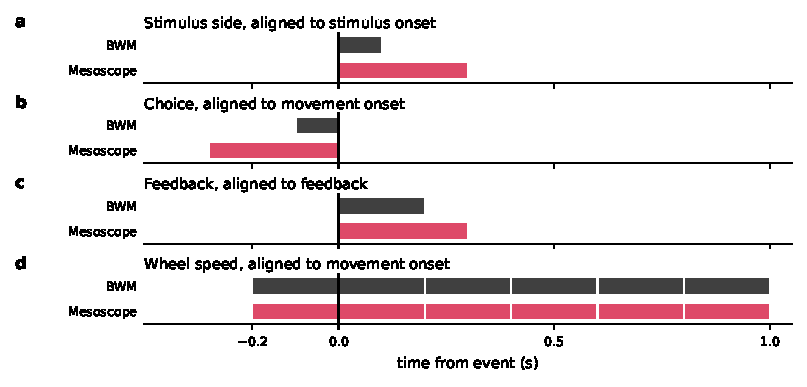
\includegraphics[width=5.35in,height=0.8\textheight,keepaspectratio]{figures/windows.pdf}
  \caption{Analysis windows used for decoding and for the single-neuron tuning test. BWM windows follow the Brain Wide Map single-cell analyses. Mesoscope frames are about 0.2\,s apart, so the mesoscope stimulus, choice and feedback windows are widened to 0.3\,s to always contain at least one frame; the mesoscope value is the mean of the deconvolved trace, linearly interpolated at each neuron's own sampling times, over the window. BWM values are firing rates (spike count / window length). \textbf{a} Stimulus side: activity in window $[0, 0.1]$\,s (BWM) or $[0, 0.3]$\,s (mesoscope) relative to stimulus onset. \textbf{b} Choice: window $[-0.1, 0]$\,s (BWM) or $[-0.3, 0]$\,s (mesoscope) relative to movement onset. \textbf{c} Feedback: window $[0, 0.2]$\,s (BWM) or $[0, 0.3]$\,s (mesoscope) relative to feedback. \textbf{d} Wheel speed: six 0.2\,s bins from $-0.2$ to $1$\,s around movement onset, identical for both modalities; each bin's activity is paired with the mean absolute wheel velocity in the same bin.}
  \label{fig:windows}
\end{figure}


\section*{Methods}
\paragraph{Data selection.}
\begin{itemize}
  \item \textbf{Mesoscope:} 151 of the 165 canonical sessions (see below). Neurons are ROIs classified as neurons, labelled isocortex (Allen Cosmos level) and with a valid position. Activity is the deconvolved trace.
  \item \textbf{BWM:} 2023 release, 351 insertions in 288 sessions. Only good units labelled isocortex are used; activity is the firing rate (spike count / window length).
  \item \textbf{Excluded mesoscope sessions:} two sessions whose task and imaging clocks disagree. In both, the cross-correlation of population activity with wheel speed peaks at $-146$\,s and $-338$\,s instead of near 0, and every variable decodes at chance. Trials outside the imaging period are dropped (19 trials of one further session).
  \item \textbf{Trials:} BWM criteria for both datasets: all event times present, a choice was made, and reaction time between 0.08 and 2\,s. Sessions need at least 50 such trials (median 347 for the mesoscope and 414 for BWM).
  \item \textbf{Spatial bins:} each neuron is assigned to one hexagonal bin by its ML--AP Allen CCF position relative to bregma, 1\,mm across. For decoding, both hemispheres are folded onto the right one.
  \item \textbf{Depth:} depth below the pial surface is the Allen top surface at the unit's ML--AP position minus its DV. Histology-registered mesoscope sessions image 174--318\um{} deep (5--95\%). The depth-limited BWM set keeps units within 640\um.
\end{itemize}

\paragraph{Features and targets.}
\begin{itemize}
  \item One value per neuron and trial: its mean activity in the window. For the mesoscope, each neuron's trace is linearly interpolated at its own sampling times, which include the per-plane time offset, before averaging.
  \item \textbf{Stimulus side:} left vs right, including 0\% contrast trials. \textbf{Choice:} left vs right wheel turn. \textbf{Feedback:} reward vs error.
  \item \textbf{Wheel speed:} mean absolute wheel velocity in each of six 0.2\,s bins, paired with the activity in the same bin. All bins of all trials are decoded together.
\end{itemize}

\paragraph{Decoders and cross-validation.}
\begin{itemize}
  \item A separate decoder is fit for every session $\times$ bin, using either all neurons of that session in the bin or a random draw of 20 neurons (bins with at least 20 neurons, mean over 10 draws).
  \item \textbf{Outer loop:} 5-fold cross-validation over trials, with the same folds for every bin of a session. For binary targets the folds are stratified by class. Features are z-scored using training trials only.
  \item \textbf{Binary targets:} L2-regularised logistic regression with balanced class weights. The regularisation strength (6 values, $C$ from $10^{-4}$ to 10) is chosen by an inner 3-fold cross-validation on the training trials, maximising balanced accuracy. The score is the balanced accuracy of the pooled held-out predictions (chance 0.5).
  \item \textbf{Wheel speed:} ridge regression; the penalty (7 values, 0.1 to $10^5$) is chosen by exact leave-one-trial-out error (rows of a trial are correlated), and the activity of the previous, same and next 0.2\,s bin are the features for each wheel bin. Folds keep all bins of a trial together. The score is the $R^2$ of the pooled held-out predictions (chance 0). Trial-specific wheel speed subtracts the per-bin mean speed of the training trials from the target.
  \item The decoders run on the GPU and reproduce scikit-learn's \texttt{LogisticRegressionCV} and \texttt{RidgeCV} pipelines. For sets with more neurons than trials, the logistic decoders are fit in the row space of the trials, which is exact.
\end{itemize}

\paragraph{Averaging.}
\begin{itemize}
  \item \textbf{Decoding maps:} the value of a bin is the mean score over all sessions that contribute at least 20 neurons to it.
  \item \textbf{Scatter plots:} the same per-bin means, for the bins covered by both datasets.
  \item \textbf{Headline numbers:} means over all session $\times$ bin pairs.
  \item \textbf{Tuning maps:} neurons are pooled across sessions within a bin; the value is the fraction with $p < 0.05$, shown for bins with at least 10 neurons.
\end{itemize}

\paragraph{Single-neuron tuning test.}
\begin{itemize}
  \item The BWM single-cell test, applied to the same windows. Mann--Whitney $U$ statistics compare the two conditions within strata (block $\times$ choice for stimulus side, block $\times$ stimulus side for choice and feedback), summed and normalised.
  \item The null distribution comes from 3{,}000 permutations of the condition labels within consecutive blocks, and $p$ is the rank of the observed statistic. Zero-contrast trials do not enter this test.
  \item Sessions without biased blocks (55 mesoscope sessions) are tested within their single 0.5 block. Neurons that cannot be tested are left out of the fractions.
\end{itemize}

\paragraph{Region and session variance (\figref{region_variance}).}
\begin{itemize}
  \item \textbf{Mesoscope scores:} one all-neuron score per session and Beryl region (all neurons of the session in the region, at least 20), with the decoders of \figref{decoding_all}.
  \item \textbf{BWM per probe:} one score per probe from all its isocortex units (at least 20), assigned to the Beryl region 300\um{} below its brain entry point (histology-aligned trajectory). Angled probes drift, so this is the majority region of the probe's superficial units for only about two thirds of probes.
  \item \textbf{BWM decoding paper:} the published Brain Wide Map decoding results (stage-2 tables), one score per session and region from all units of the region, with no minimum unit count (median 16). Each score comes with a $p$-value against 100--200 pseudo-sessions and the median of that null, which is the baseline in \figref{region_variance}. These tables have wheel velocity instead of trial-specific wheel speed.
  \item \textbf{Regions:} the 15 with at least 3 mesoscope sessions and 3 BWM probes.
  \item \textbf{Shuffle control (mesoscope, BWM per probe):} the same decoders with the trials of all labels and of wheel speed permuted jointly, neural data untouched; 1 permutation per mesoscope score and 3 per probe, pooled per region. This plain trial permutation is less strict than the pseudo-session null of the decoding paper, which keeps the block structure, so the band can sit slightly lower, mainly for stimulus side and choice. For wheel speed the shuffled $R^2$ is not zero: the stereotyped speed profile after movement onset is still predicted from the stereotyped neural time course.
  \item \textbf{Statistics, mesoscope only.} In BWM nearly every session has one probe, so session variance cannot be separated from probe-to-probe variance. The decoding-paper tables do not help either: few sessions have scores in two or more of these regions, and those regions are usually adjacent along one probe. All-neuron scores grow with the number of neurons, so log neuron count is a covariate in the mixed model and is regressed out before the permutation tests.
  \item \textbf{Mixed model:} score $\sim$ log $N$ + (1$|$region) + (1$|$animal) + (1$|$session), crossed random effects, REML (statsmodels). Each component's share is its variance over the total, and each is tested by a likelihood-ratio test against the model without it ($\chi^2_{0/1}$ mixture).
  \item \textbf{Permutation tests:} the same question without a statistical model, using only reshuffling, on the scores with log $N$ regressed out.
  \begin{itemize}
    \item \emph{Region:} each session's mean is subtracted from its region scores, so a good session or animal cannot make its regions look good. The statistic is $\eta^2$, the share of the remaining variance that lies between regions. The null comes from 5{,}000 shuffles of the region labels within each session (sessions with at least 2 regions).
    \item \emph{Session:} the mirror image. Each region's mean is subtracted, $\eta^2$ is the share between sessions, and session labels are shuffled within each region.
    \item $\eta^2$ is above 0 even for random labels, and more so with many groups (about 150 sessions vs 15 regions). The figure therefore shows adjusted $\eta^2$ = ($\eta^2 -$ null mean) / (1 $-$ null mean): 0 is chance level and positive values are the share beyond chance. $p$ is the fraction of shuffles with $\eta^2$ at least as large as observed.
  \end{itemize}
\end{itemize}

\section*{Headline numbers}
\begin{table}[!htbp]
\centering\small
\begin{tabular}{lrrr}
\toprule
 & Mesoscope & BWM $\leq$640\um & BWM all depths \\
\midrule
Isocortex neurons (sessions) & 1{,}071{,}534 (151) & 2{,}929 (204) & 13{,}002 (288) \\
Session $\times$ bin pairs with $\geq$20 neurons & 1{,}763 & 54 & 216 \\
Median neurons per session $\times$ bin ($\geq$20) & 458 & 27 & 40 \\
Fraction tuned: stimulus side / choice / feedback & 0.147 / 0.107 / 0.254 & 0.075 / 0.090 / 0.233 & 0.069 / 0.108 / 0.294 \\
Stimulus side, 20 neurons / all & 0.542 / 0.620 & 0.538 / 0.546 & 0.541 / 0.551 \\
Choice, 20 neurons / all & 0.527 / 0.585 & 0.599 / 0.615 & 0.621 / 0.655 \\
Feedback, 20 neurons / all & 0.650 / 0.819 & 0.632 / 0.651 & 0.691 / 0.738 \\
Wheel speed $R^2$, 20 neurons / all & 0.046 / 0.215 & 0.246 / 0.286 & 0.306 / 0.385 \\
Trial-specific wheel speed $R^2$, 20 neurons / all & 0.012 / 0.076 & 0.052 / 0.065 & 0.073 / 0.110 \\
Bin-means-only wheel $R^2$ (no neurons, median session) & 0.47 & 0.44 & 0.44 \\
\bottomrule
\end{tabular}
\caption*{Decoding: balanced accuracy (chance 0.5) or $R^2$ (chance 0), mean over session $\times$ bin pairs. ``All'' uses every neuron of a session in the bin; mesoscope bins hold about 20 times more neurons, so only the 20-neuron columns compare like with like. Only 53 of the 204 sessions with superficial BWM units have a bin with at least 20 of them.}
\end{table}

\FloatBarrier
\section*{Maps}
Coverage at 1\,mm. The depth-limited BWM row is sparse: most bins hold one or two sessions (\figref{counts}).

\begin{figure}[!htbp]
  \centering
  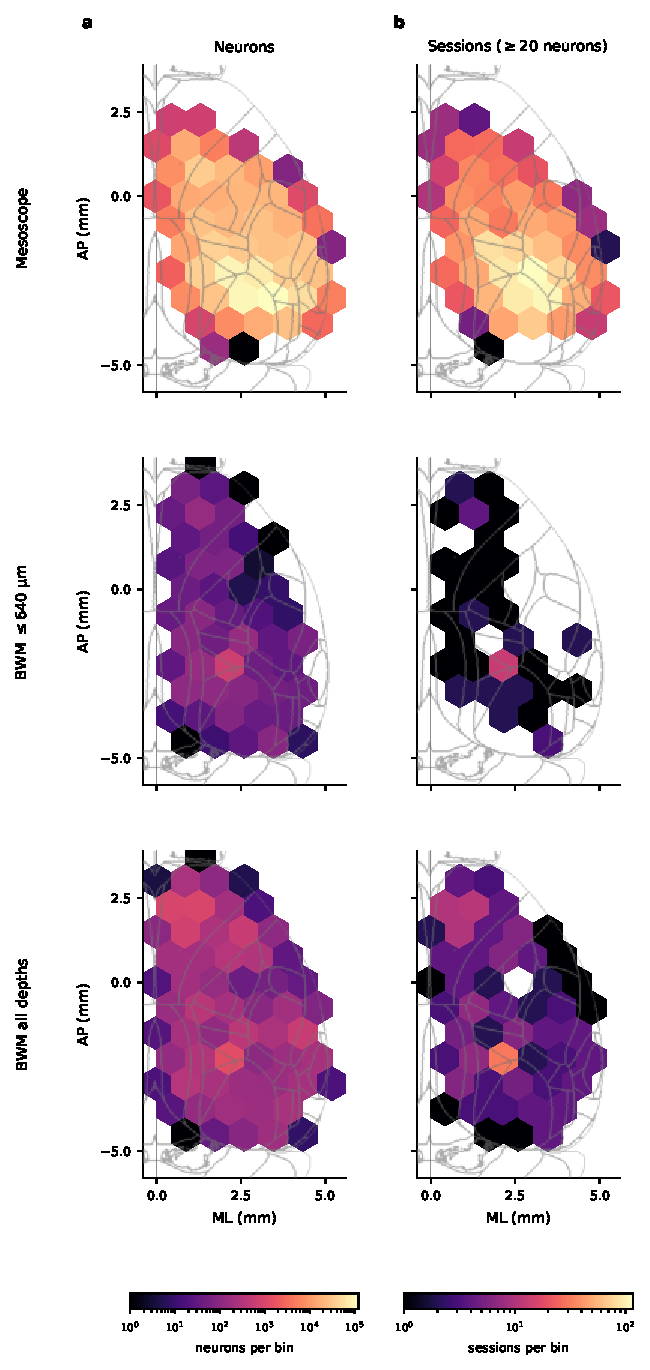
\includegraphics[width=4.32in,height=0.8\textheight,keepaspectratio]{figures/counts.pdf}
  \caption{Coverage: mesoscope two-photon imaging (top row; deconvolved activity of isocortex neurons) vs Brain Wide Map Neuropixels units within 640\,$\mu$m of the pial surface (middle row; twice the depth range the mesoscope images, 174--318\,$\mu$m) and at all depths (bottom row; reference). Each neuron is assigned to a hexagonal bin (1\,mm vertex to vertex) by its ML and AP Allen CCF position; hemispheres folded onto the right. Grey lines: Allen top-view region boundaries. Colour scales are shared across rows. \textbf{a} Number of isocortex neurons per bin: mesoscope 1,071,534 neurons, 151 sessions; BWM $\leq$640\,$\mu$m 2,929 neurons, 204 sessions; BWM all depths 13,002 neurons, 288 sessions. \textbf{b} Number of sessions contributing at least 20 neurons to each bin.}
  \label{fig:counts}
\end{figure}


Fraction of tuned neurons. The mesoscope still has about twice as many stimulus-side-tuned neurons as BWM, whether or not BWM is restricted to superficial units (\figref{tuning}).

\begin{figure}[!htbp]
  \centering
  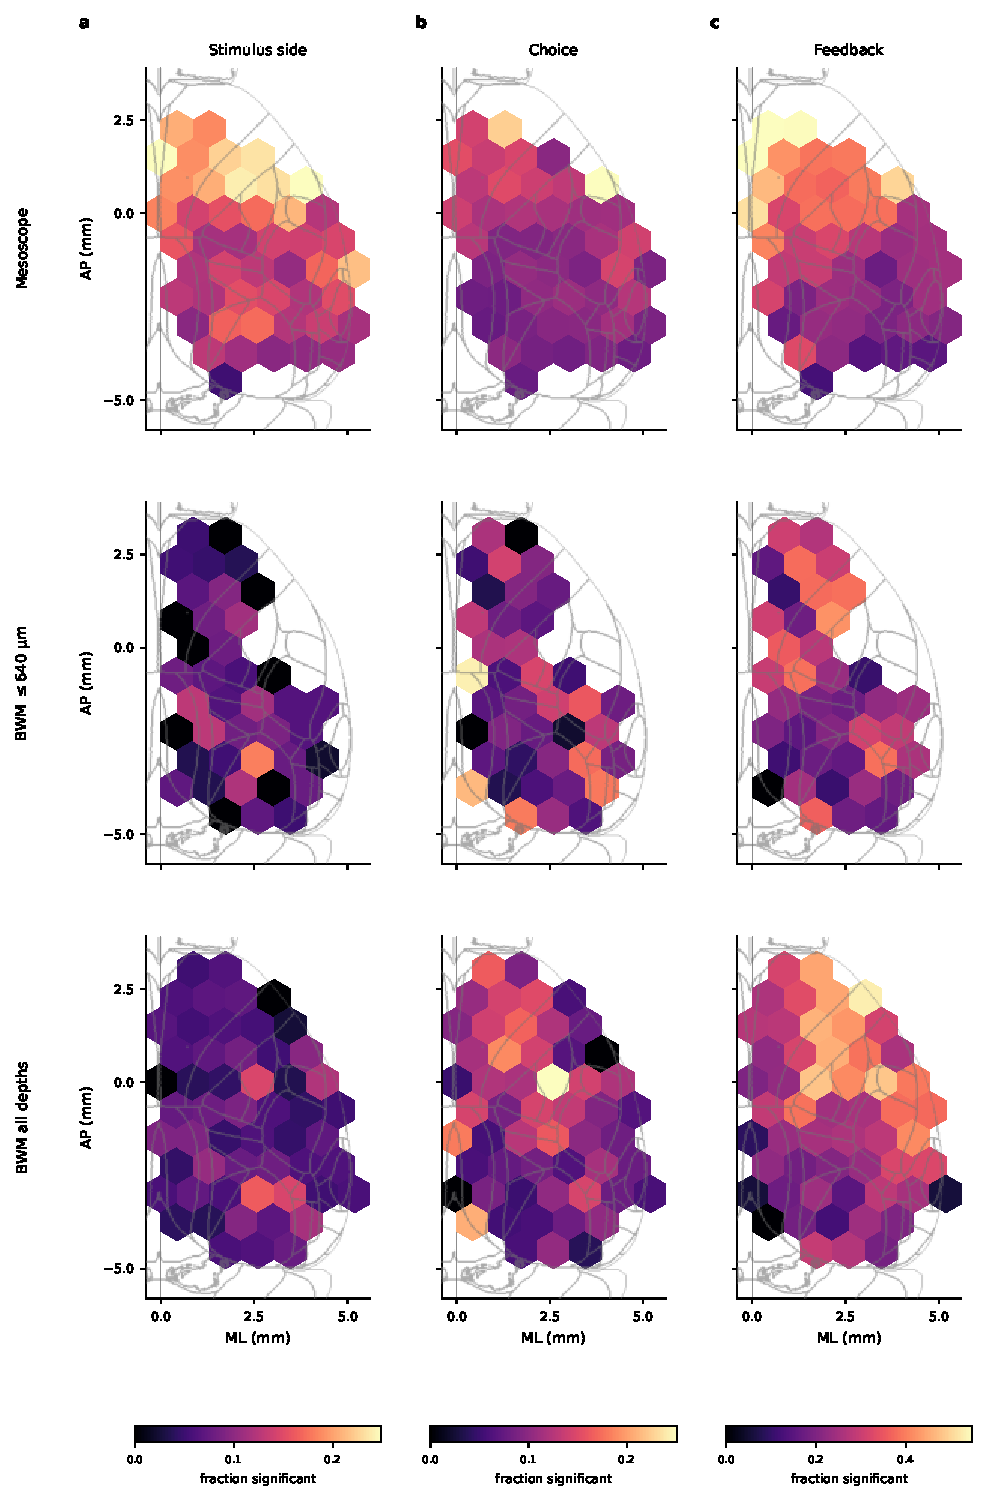
\includegraphics[width=\linewidth,height=0.8\textheight,keepaspectratio]{figures/tuning.pdf}
  \caption{Tuning results: mesoscope two-photon imaging (top row; deconvolved activity of isocortex neurons) vs Brain Wide Map Neuropixels units within 640\,$\mu$m of the pial surface (middle row; twice the depth range the mesoscope images, 174--318\,$\mu$m) and at all depths (bottom row; reference). Each neuron is assigned to a hexagonal bin (1\,mm vertex to vertex) by its ML and AP Allen CCF position; hemispheres folded onto the right. Grey lines: Allen top-view region boundaries. Colour scales are shared across rows. Single-neuron tuning: the BWM single-cell test (brainwidemap single\_cell\_stats, re-implemented on the GPU and checked against the original), applied identically to both modalities to the mean activity in each window. Mann--Whitney $U$ statistics are computed within condition strata, summed and normalised; the null distribution comes from 3000 permutations of the condition labels within consecutive blocks, and $p$ is the rank of the observed statistic. Mesoscope windows are 0.3\,s long because the frame period is about 0.2\,s. \textbf{a} Fraction of neurons per bin tuned to stimulus side ($p<0.05$; bins with $\geq$10 neurons pooled across sessions); window $[0, 0.1]$\,s (BWM) or $[0, 0.3]$\,s (mesoscope) relative to stimulus onset. \textbf{b} Choice; window $[-0.1, 0]$\,s (BWM) or $[-0.3, 0]$\,s (mesoscope) relative to movement onset. \textbf{c} Feedback; window $[0, 0.2]$\,s (BWM) or $[0, 0.3]$\,s (mesoscope) relative to feedback.}
  \label{fig:tuning}
\end{figure}


Decoding from 20 random neurons per session and bin (mean over 10 draws), so all three rows are compared at the same population size; only sessions with at least 20 neurons in a bin enter it. Stimulus side, choice and feedback are decoded with L2 logistic regression in the windows of \figref{windows} (balanced accuracy, chance 0.5). Wheel speed uses the revised decoder: ridge regression on the activity of the previous, same and next 0.2\,s bin, scored by cross-validated $R^2$. Trial-specific wheel speed subtracts the mean speed profile of the training trials, so only trial-to-trial differences in speed count. Bins fade when fewer than four animals contribute (\figref{decoding_n20}).

\begin{figure}[!htbp]
  \centering
  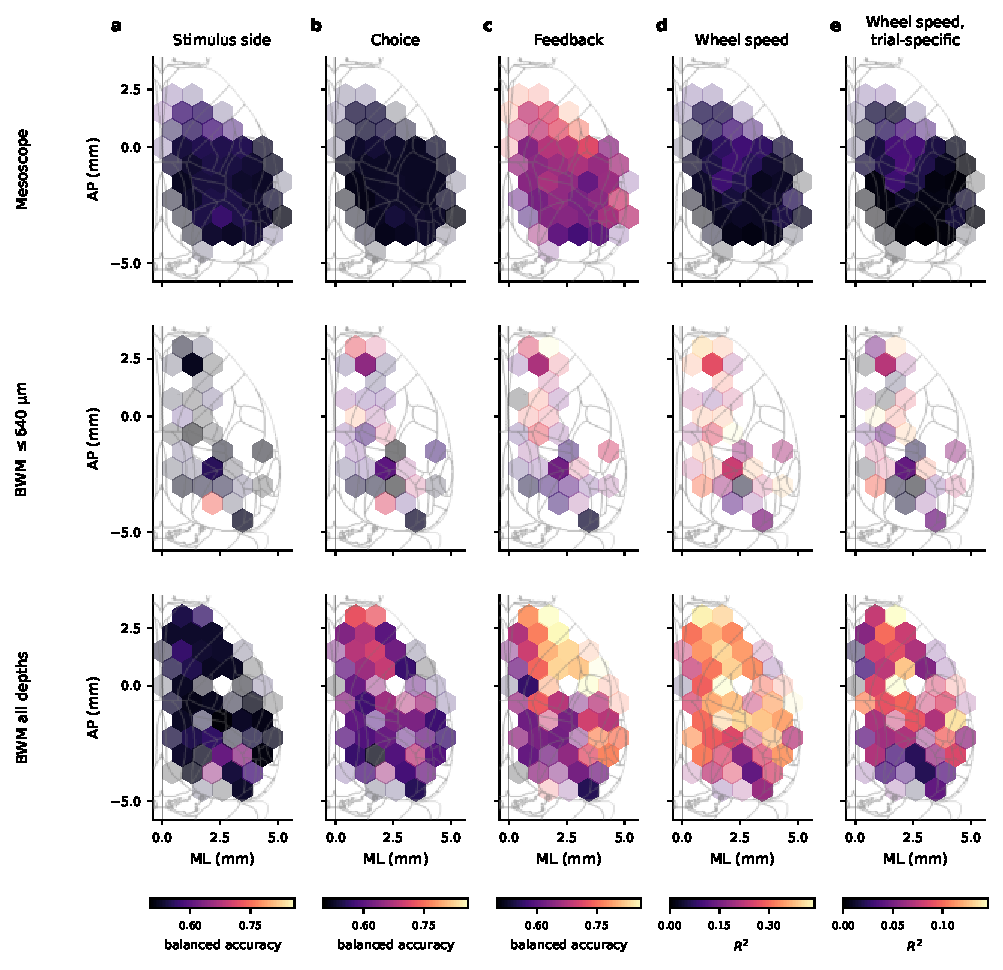
\includegraphics[width=\linewidth,height=0.8\textheight,keepaspectratio]{figures/decoding_n20.pdf}
  \caption{\textbf{Decoding from 20 neurons}. Rows: mesoscope; BWM units within 640\,$\mu$m of the pial surface; BWM at all depths. Each bin (1\,mm hexagon, hemispheres folded) shows the mean over sessions of decoders trained on 20 random neurons of one session in that bin (mean of 10 draws; sessions with $\geq$20 neurons there). Opacity: number of animals (full at $\geq$4). \textbf{a} Stimulus side, balanced accuracy (chance 0.5; colour scale shared by \textbf{a}--\textbf{c}). \textbf{b} Choice. \textbf{c} Feedback. \textbf{d} Wheel speed, cross-validated $R^2$. \textbf{e} Trial-specific wheel speed, $R^2$.}
  \label{fig:decoding_n20}
\end{figure}


Decoding from all neurons of a session in a bin, otherwise as in \figref{decoding_n20}. Mesoscope bins hold about 20 times more neurons than BWM bins (median 458 vs 27), so the rows are not comparable in absolute terms. With hundreds of neurons per bin, the mesoscope decodes stimulus side and feedback better than BWM, and its frontal feedback map stands out. The bottom row decodes each BWM probe from all its isocortex units and places it at its brain entry point; per-probe medians match the per-bin ones (\figref{decoding_all}).

\begin{figure}[!htbp]
  \centering
  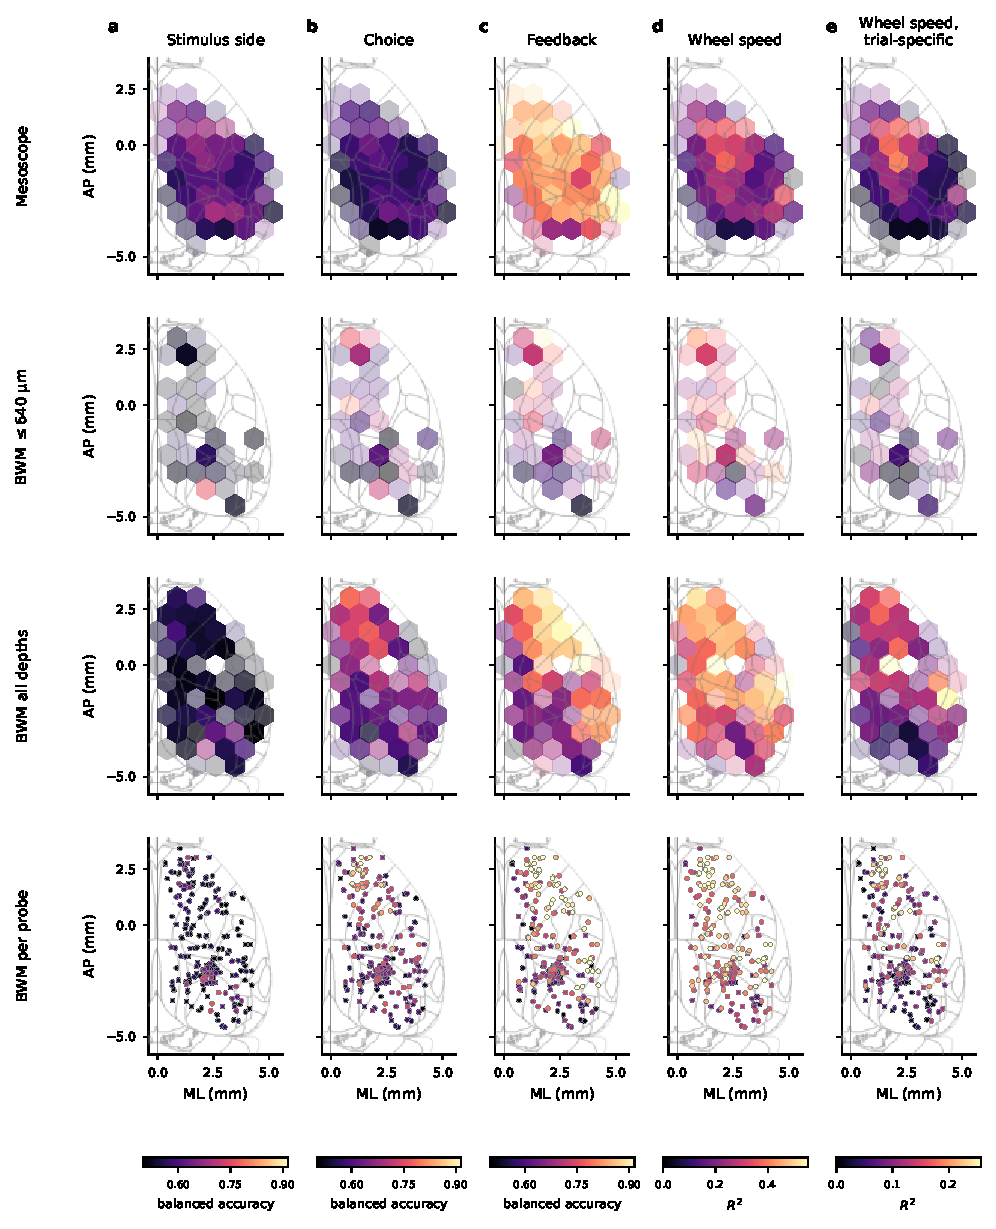
\includegraphics[width=\linewidth,height=0.8\textheight,keepaspectratio]{figures/decoding_all.pdf}
  \caption{\textbf{Decoding from all neurons}. Rows: mesoscope; BWM units within 640\,$\mu$m of the pial surface; BWM at all depths. Each bin (1\,mm hexagon, hemispheres folded) shows the mean over sessions of decoders trained on all neurons of one session in that bin (sessions with $\geq$20 neurons there); mesoscope bins hold far more neurons than BWM bins. Opacity: number of animals (full at $\geq$4). Bottom row: BWM decoded per probe from all its isocortex units at all depths, whichever bins they fall in (209 probes with $\geq$20 units, median 40); each circle sits at the probe's brain entry point (histology-aligned Alyx trajectory, hemispheres folded), higher scores drawn on top where circles overlap; colour scales as in the rows above, so circles beyond the top of a scale saturate. \textbf{a} Stimulus side, balanced accuracy (chance 0.5; colour scale shared by \textbf{a}--\textbf{c}). \textbf{b} Choice. \textbf{c} Feedback. \textbf{d} Wheel speed, cross-validated $R^2$. \textbf{e} Trial-specific wheel speed, $R^2$.}
  \label{fig:decoding_all}
\end{figure}


\FloatBarrier
\section*{Variance across regions and sessions}
Do all-neuron scores differ more between regions or between sessions? Scores are shown per Beryl region for the mesoscope (per session), BWM per probe (at its entry region) and the BWM decoding paper (per session and region), for the 15 regions sampled by both datasets. In both BWM versions frontal motor cortex stands out: MOp and MOs have the highest median scores for choice, feedback and wheel speed in the decoding paper. In the mesoscope, where every session samples several regions, region matters (mixed model, region share 10--30\%, all $p<0.001$, most for wheel speed), but sessions and animals together account for more (41--59\%). The model-free test agrees: within a region, scores vary more across sessions than across regions within a session, for every variable. For ephys we do not have enough data to test how much region and session contribute to the variance: few BWM sessions record two or more of these regions, and those are usually adjacent along one probe. The two BWM rows of \figref{region_variance}a therefore only show the scores, and panels b and c are mesoscope only.

\begin{figure}[!htbp]
  \centering
  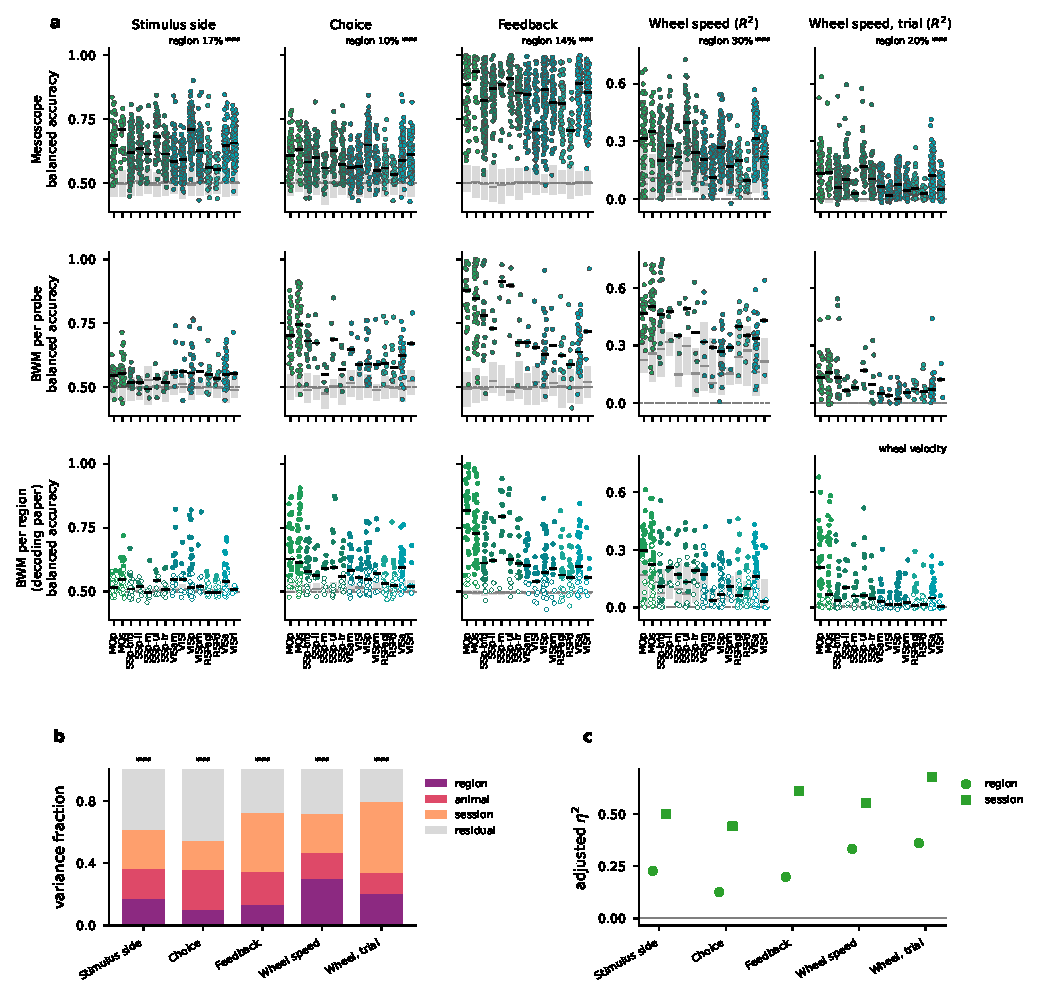
\includegraphics[width=\linewidth,height=0.8\textheight,keepaspectratio]{figures/region_variance.pdf}
  \caption{\textbf{Variance of decoding across regions and sessions (all neurons).} The 15 regions with $\geq$3 mesoscope sessions and BWM probes. Methods: \emph{Region and session variance}. \textbf{a} Scores per region (columns ordered as in the Allen structure tree; Allen colours; bar: median; dashed: chance; grey band and line: 5--95th percentile and median of the baseline; for trial-specific wheel speed the shuffle baseline lies at $R^2 \approx 0$ and is hidden by the dashed line). Top: mesoscope, one dot per session and region from all its neurons there (149 sessions, 12 animals); baseline: shuffle control. Middle: BWM, one dot per probe from all its isocortex units, placed in the region where it enters the brain (198 probes, 93 animals; the majority region of its superficial units for 66\% of probes); baseline: shuffle control. Bottom: BWM decoding paper, one dot per session and region from the region's units (346 pairs, 263 sessions, 116 animals); filled: $p<0.05$ against pseudo-sessions (21--70\% of dots); baseline: median of the pseudo-session null; wheel velocity in place of trial-specific wheel speed. Y axes shared within balanced accuracy and within $R^2$. Inset, top row: region share of variance from \textbf{b}. \textbf{b} Mesoscope variance fractions from a mixed model, score $\sim$ log $N$ + (1$|$region) + (1$|$animal) + (1$|$session); stars: likelihood-ratio test of the region component. Region: stimulus side 17\%, choice 10\%, feedback 14\%, wheel speed 30\%, wheel, trial 20\%; session plus animal: stimulus side 45\%, choice 44\%, feedback 58\%, wheel speed 41\%, wheel, trial 59\%. \textbf{c} The same question as \textbf{b}, do scores differ more between regions or between sessions, but without a statistical model, using only reshuffling: adjusted $\eta^2$ of region (circles, within sessions) and of session (squares, within regions), 0 = chance. Filled: $p<0.05$.}
  \label{fig:region_variance}
\end{figure}


\FloatBarrier
\section*{Summary and bin-wise agreement}
Top: mean scores per row. Bottom: per-bin mesoscope against depth-limited BWM, for the 25 bins covered by both (20 neurons), with spatial-null $p$-values. Wheel speed and feedback agree best ($r_s$ 0.32 and 0.30), but nothing survives the spatial null ($p_\text{sp} \geq 0.12$; \figref{summary}).

\begin{figure}[!htbp]
  \centering
  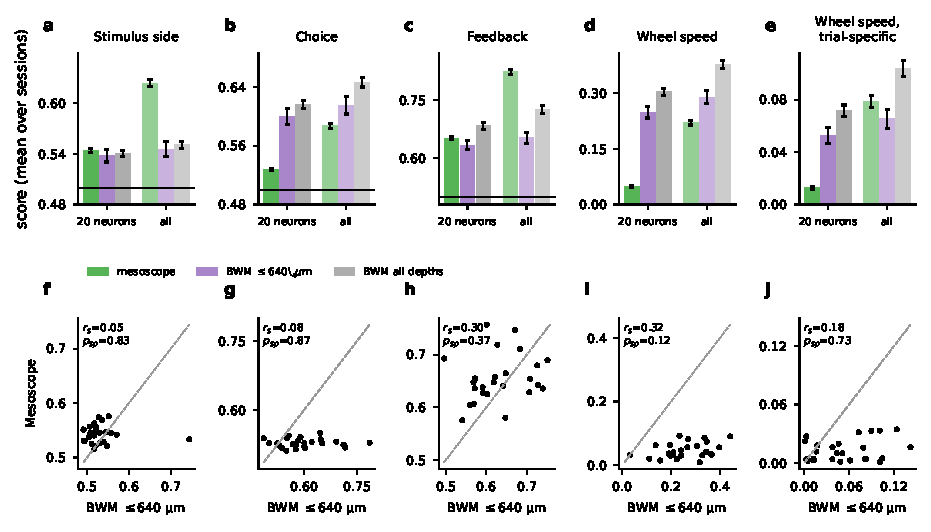
\includegraphics[width=\linewidth,height=0.8\textheight,keepaspectratio]{figures/summary.pdf}
  \caption{Summary of the revised decoding. \textbf{a--e} Mean over sessions ($\pm$ s.e.m.) of each session's mean score over its 1\,mm bins, from 20 random neurons (left, solid) and all neurons (right, light). \textbf{f--j} Per 1\,mm bin, 20 neurons: BWM $\leq$640\,$\mu$m (x) vs mesoscope (y), the 25 bins covered by both; Spearman $r_s$, naive $p$, and $p_{sp}$ against 1000 variogram-matched surrogates of either map (larger $p$ reported). Decoding per session and bin (sessions with $\geq$50 trials and $\geq$20 neurons in the bin), 5-fold cross-validation over trials. Binary variables: L2 logistic regression, balanced accuracy (chance 0.5). Wheel speed in six 0.2\,s bins from $-0.2$ to $1$\,s around movement onset: ridge regression on the activity of the previous, same and next bin (penalty by exact leave-one-trial-out error), cross-validated $R^2$; trial-specific: the same with the mean speed profile of the training trials subtracted, so only trial-to-trial differences in speed count. \textbf{a} Stimulus side, 20 neurons: mesoscope 0.544, BWM $\leq$640\,$\mu$m 0.538, BWM all depths 0.541; all neurons: mesoscope 0.624, BWM $\leq$640\,$\mu$m 0.546, BWM all depths 0.551. \textbf{b} Choice, 20 neurons: mesoscope 0.527, BWM $\leq$640\,$\mu$m 0.600, BWM all depths 0.616; all neurons: mesoscope 0.587, BWM $\leq$640\,$\mu$m 0.615, BWM all depths 0.647. \textbf{c} Feedback, 20 neurons: mesoscope 0.652, BWM $\leq$640\,$\mu$m 0.633, BWM all depths 0.683; all neurons: mesoscope 0.822, BWM $\leq$640\,$\mu$m 0.652, BWM all depths 0.726. \textbf{d} Wheel speed, 20 neurons: mesoscope 0.048, BWM $\leq$640\,$\mu$m 0.248, BWM all depths 0.303; all neurons: mesoscope 0.220, BWM $\leq$640\,$\mu$m 0.289, BWM all depths 0.377. \textbf{e} Wheel speed, trial-specific, 20 neurons: mesoscope 0.013, BWM $\leq$640\,$\mu$m 0.053, BWM all depths 0.072; all neurons: mesoscope 0.079, BWM $\leq$640\,$\mu$m 0.065, BWM all depths 0.104. \textbf{f} Stimulus side: $r_s$ = 0.05, naive $p$ = 0.80, $p_{sp}$ = 0.83. \textbf{g} Choice: $r_s$ = 0.08, naive $p$ = 0.69, $p_{sp}$ = 0.87. \textbf{h} Feedback: $r_s$ = 0.30, naive $p$ = 0.15, $p_{sp}$ = 0.37. \textbf{i} Wheel speed: $r_s$ = 0.32, naive $p$ = 0.11, $p_{sp}$ = 0.12. \textbf{j} Wheel speed, trial-specific: $r_s$ = 0.18, naive $p$ = 0.38, $p_{sp}$ = 0.73.}
  \label{fig:summary}
\end{figure}


\FloatBarrier
\section*{Does depth explain the differences?}
BWM tuning and wheel correlation per 160\um{} depth band, with the mesoscope level as a green line. Choice and feedback tuning rise in deep layers, which the 640\um{} cutoff mostly excludes. The fraction of wheel-correlated units is 20--25\% at every depth, against 4\% of mesoscope neurons, so depth does not explain the mesoscope's weak wheel decoding (\figref{depth}).

\begin{figure}[!htbp]
  \centering
  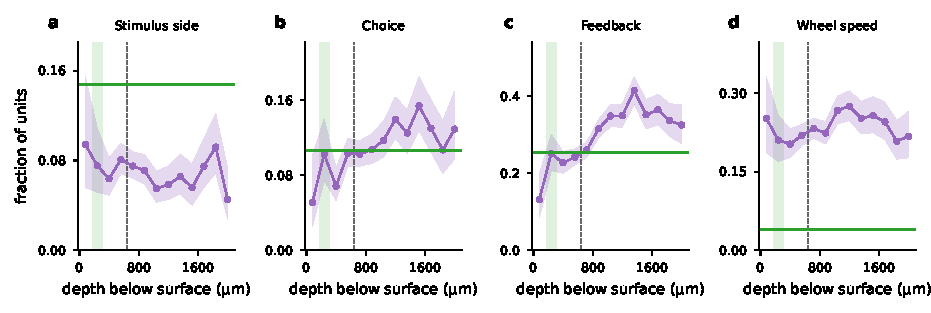
\includegraphics[width=\linewidth,height=0.8\textheight,keepaspectratio]{figures/depth.pdf}
  \caption{Depth sensitivity of the BWM comparison. Green line: mesoscope fraction over all neurons; green shading: mesoscope imaging depth (174--318\,$\mu$m, 5--95\,\% of the histology-registered sessions); dashed line: the 640\,$\mu$m cutoff of the depth-limited BWM set. Depth: Allen CCF top surface at the unit's ML-AP position minus its DV. \textbf{a} Fraction of BWM isocortex units tuned to stimulus side ($p<0.05$, same test as the maps) per 160\,$\mu$m depth band (purple; band: 95\,\% Wilson interval; bands with $\geq$30 units): 7.5\% of BWM units within 640\,$\mu$m, 6.7\% deeper, mesoscope 14.7\%. \textbf{b} Choice: 9.0\% of BWM units within 640\,$\mu$m, 11.4\% deeper, mesoscope 10.7\%. \textbf{c} Feedback: 23.3\% of BWM units within 640\,$\mu$m, 31.2\% deeper, mesoscope 25.4\%. \textbf{d} Fraction of units correlated with wheel speed ($r>0.1$ over the wheel bins of both the even and the odd trials): 21.5\% of BWM units within 640\,$\mu$m, 23.2\% deeper, mesoscope 4.0\%.}
  \label{fig:depth}
\end{figure}


\FloatBarrier
\section*{Wheel-speed decoding revisited}
Rasters first: wheel speed in the six wheel bins of 30 consecutive trials, above the 60 neurons most correlated with it. Neurons are ranked on the other trials of the session, so the trials shown are held out. The middle and right columns show the same 60 neurons, row for row: their trial-averaged activity per bin and their $r$ with wheel speed. In the two best mesoscope sessions, the mean of these neurons (coloured trace) follows wheel speed at $r = 0.58$ and 0.53, comparable to the best BWM sessions (0.29 and 0.63). But they are a small minority: only 1--18\% of mesoscope neurons reach $r > 0.1$ in these sessions, against 0--42\% in BWM (\figref{rasters}).

\begin{figure}[!htbp]
  \centering
  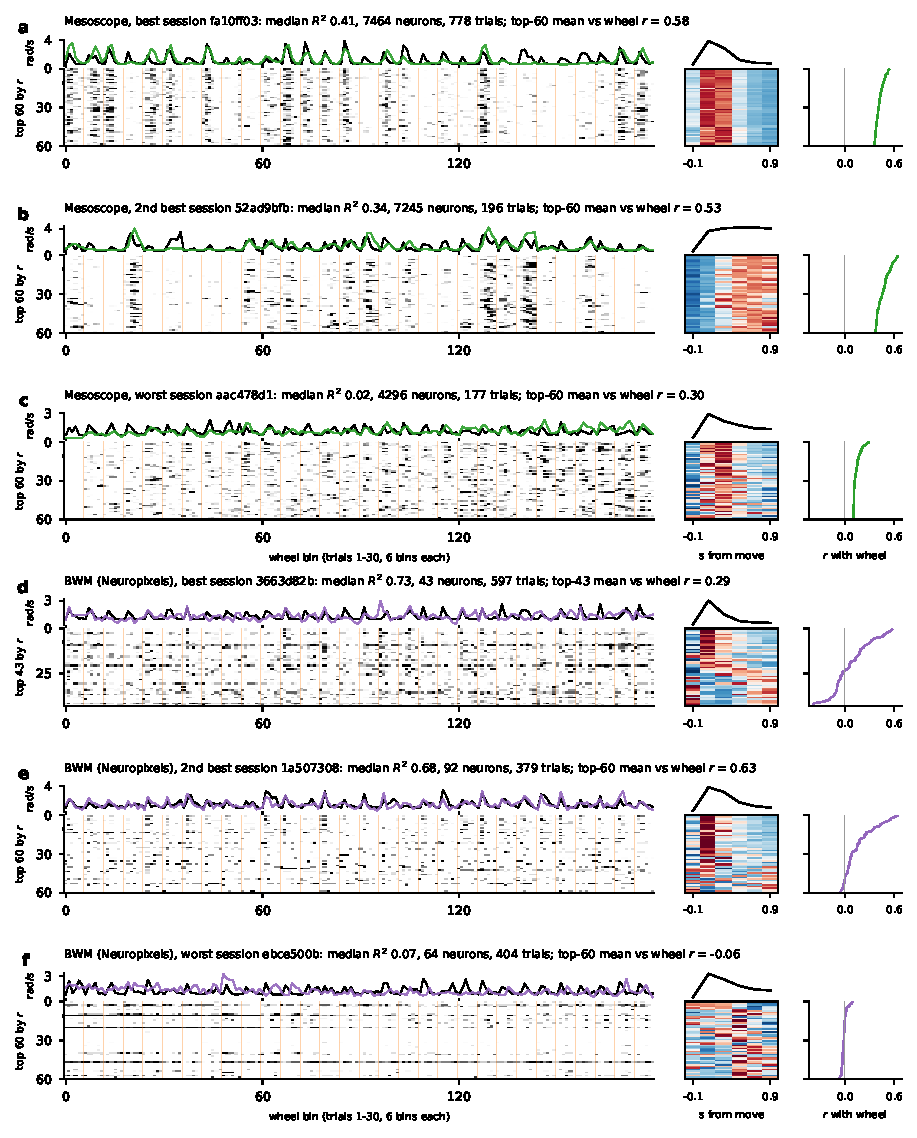
\includegraphics[width=\linewidth,height=0.8\textheight,keepaspectratio]{figures/rasters.pdf}
  \caption{Neural correlates of wheel speed. Each row: wheel speed (top; rad/s) in the 6 wheel bins (0.2\,s, $-0.2$ to 1\,s around first movement) of the first 30 trials, concatenated (orange lines: trial boundaries; bins are not contiguous across trials; coloured: mean z-scored activity of the neurons below, rescaled), above the z-scored activity of the 60 neurons most positively correlated with wheel speed (sorted by $r$, highest on top). Neurons are ranked by $r$ over all bins of the remaining trials, so the shown trials are held out from the selection. Middle: trial-averaged activity of the same 60 neurons per bin (z-scored per neuron, same order), with the mean wheel speed above. Right: their $r$ with wheel speed over the remaining trials, same rows. Sessions at the best two and the worst of each modality by the session median $R^2$ over bins (all neurons per 0.4\,mm bin, revised decoder with lagged features; sessions with $\geq$30 neurons). \textbf{a} Mesoscope session fa10ff03 (best of 149 sessions by the session median wheel-speed $R^2$): 95th percentile of $r$ over neurons 0.20, maximum 0.54, 17\% of neurons with $r>0.1$; mean of the top 60 neurons vs wheel speed in the shown trials $r$ = 0.58. \textbf{b} Mesoscope session 52ad9bfb (2nd best of 149 sessions by the session median wheel-speed $R^2$): 95th percentile of $r$ over neurons 0.20, maximum 0.64, 18\% of neurons with $r>0.1$; mean of the top 60 neurons vs wheel speed in the shown trials $r$ = 0.53. \textbf{c} Mesoscope session aac478d1 (worst of 149 sessions by the session median wheel-speed $R^2$): 95th percentile of $r$ over neurons 0.07, maximum 0.29, 1\% of neurons with $r>0.1$; mean of the top 60 neurons vs wheel speed in the shown trials $r$ = 0.30. \textbf{d} BWM (Neuropixels) session 3663d82b (best of 127 sessions by the session median wheel-speed $R^2$): 95th percentile of $r$ over neurons 0.50, maximum 0.57, 42\% of neurons with $r>0.1$; mean of the top 43 neurons vs wheel speed in the shown trials $r$ = 0.29. \textbf{e} BWM (Neuropixels) session 1a507308 (2nd best of 127 sessions by the session median wheel-speed $R^2$): 95th percentile of $r$ over neurons 0.51, maximum 0.64, 30\% of neurons with $r>0.1$; mean of the top 60 neurons vs wheel speed in the shown trials $r$ = 0.63. \textbf{f} BWM (Neuropixels) session ebce500b (worst of 127 sessions by the session median wheel-speed $R^2$): 95th percentile of $r$ over neurons 0.05, maximum 0.09, 0\% of neurons with $r>0.1$; mean of the top 60 neurons vs wheel speed in the shown trials $r$ = -0.06.}
  \label{fig:rasters}
\end{figure}


Checks: the decoder recovers an artificial neuron at the expected $R^2$, mesoscope activity lags the wheel, the $R^2$ is mostly the stereotyped speed profile, and lagged features help both modalities (\figref{checks}).

\begin{figure}[!htbp]
  \centering
  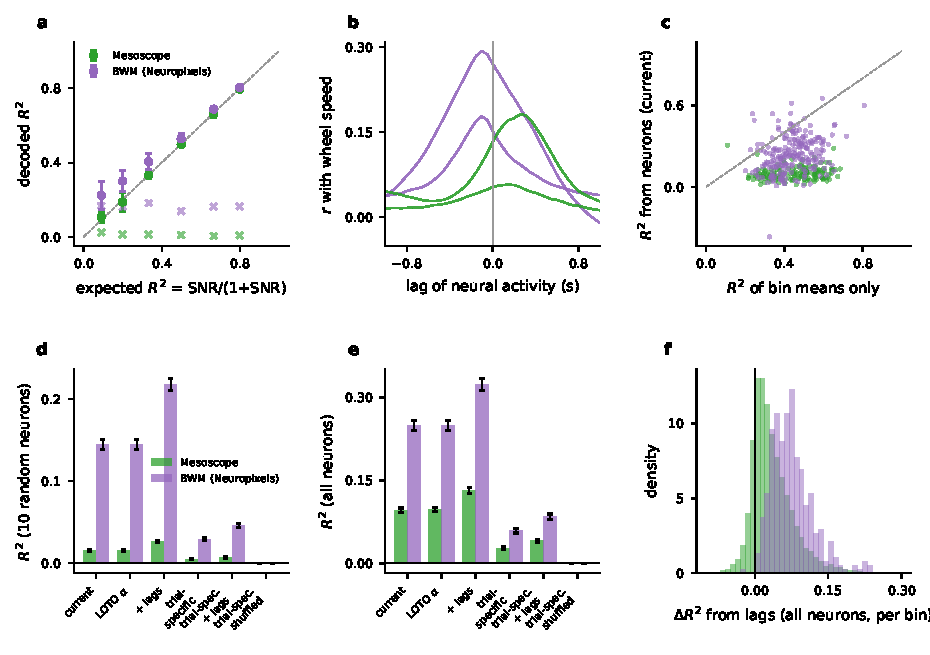
\includegraphics[width=\linewidth,height=0.8\textheight,keepaspectratio]{figures/checks.pdf}
  \caption{Checks of the wheel-speed decoding. The decoder and target are correct (after removing encoder glitches in 16 mesoscope sessions), mesoscope activity lags the wheel by about one 0.2\,s bin more than spikes, and the $R^2$ is dominated by the stereotyped speed profile after movement onset rather than by trial-to-trial differences in speed. \textbf{a} Decoder check: a synthetic neuron (wheel speed plus Gaussian noise at signal-to-noise ratios 0.1--4) replacing one of 10 random neurons of a session is recovered at the expected $R^2$ (dots: mean $\pm$ s.d. over 5 draws and 3 sessions per modality; crosses: the same 10 neurons without it). The decoder reproduces the dorsal-maps GPU decoder (max difference $2\times10^{-15}$) and the scikit-learn reference ($1\times10^{-7}$). The wheel-speed target agrees with brainbox's filtered speed ($r\geq$0.9999) once encoder glitches are removed. \textbf{b} Timing at full resolution: correlation of neural activity with wheel speed at lags $-1$ to 1\,s (positive: neural activity follows the wheel), mean over the 5\,\% most wheel-correlated neurons selected on the first half of each session and measured on the second half; 2 sessions per modality. Mesoscope deconvolved activity peaks 0.15--0.25\,s after wheel speed, BWM spikes 0.10\,s before it. \textbf{c} What the $R^2$ measures: predicting each bin from its mean over the training trials (no neural data) gives $R^2$ 0.46 (mesoscope sessions, median) and 0.44 (BWM), far above decoding from all neurons of a bin (current decoder; one dot per session). Most of the variance is the stereotyped time course after movement onset; trial-to-trial differences are 53\% (mesoscope) and 56\% (BWM) of the variance. \textbf{d} Decoder variants, 10 random neurons per 0.4\,mm bin (mean $\pm$ s.e.m. over sessions): current (leave-one-row-out choice of the ridge penalty), leave-one-trial-out (LOTO) choice, neural activity of the previous, same and next bin as features (lags), trial-specific speed (bin means of the training trials removed) without and with lags, and the trial-specific target with trials shuffled (null). Mesoscope 0.015 $\to$ 0.026 with lags, BWM 0.144 $\to$ 0.218. \textbf{e} Same from all neurons of a bin: mesoscope 0.096 $\to$ 0.132, BWM 0.249 $\to$ 0.324; trial-specific speed 0.041 vs 0.085. \textbf{f} Gain from the lagged features per (session, bin), all neurons.}
  \label{fig:checks}
\end{figure}


Across all sessions: replicable wheel correlates are rare in the mesoscope (median 3.5\% of neurons vs 22\% in BWM). The best 10 neurons of a whole session match BWM, but among 30 random neurons they fall far short of BWM ($r$ 0.15 vs 0.37) (\figref{population}).

\begin{figure}[!htbp]
  \centering
  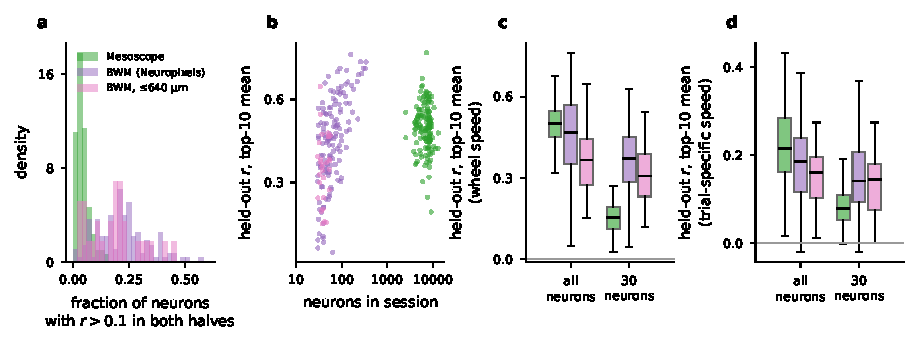
\includegraphics[width=\linewidth,height=0.8\textheight,keepaspectratio]{figures/population.pdf}
  \caption{Wheel-speed correlates are rare in the mesoscope but present: among thousands of neurons per session the best 10 track wheel speed in held-out trials as well as the best BWM units, but a random set of 30 neurons, as in a small spatial bin, contains far fewer of them than a BWM set of the same size. Sessions with $\geq$30 neurons and $\geq$50 trials. \textbf{a} Fraction of neurons per session whose correlation with wheel speed (over all wheel bins) exceeds 0.1 in both the even and the odd trials: median 3.6\% (mesoscope, 149 sessions), 21.7\% (BWM isocortex, 137), 18.2\% (BWM units within 640\,$\mu$m of the surface, 29). \textbf{b} Correlation with wheel speed in the odd trials of the mean z-scored activity of the 10 neurons that correlate best on the even trials, against the number of neurons in the session (one dot per session). \textbf{c} The same with all neurons of a session (median mesoscope 0.50, BWM 0.47, $p$ = 0.03) and with sessions subsampled to 30 random neurons (mean over 20 draws; 0.15 vs 0.37, $p<10^{-32}$). Boxes: quartiles; whiskers: 1.5 inter-quartile ranges. \textbf{d} Same against trial-specific speed (wheel speed minus its per-bin mean over the even trials): 0.22 vs 0.19 (all neurons), 0.08 vs 0.14 (30 neurons).}
  \label{fig:population}
\end{figure}


\FloatBarrier
\section*{Notes and open points}
\begin{itemize}
  \item \textbf{Tuning $p$-values.} \texttt{mpciROIs.taskTunedP} is not on Alyx and the BWM single-cell $p$-values are not in the public aggregates, so both modalities use a GPU re-implementation of the BWM single-cell test (\texttt{brainwidemap} \texttt{single\_cell\_stats}). On a 60-neuron check it agreed with the original code on $p < 0.05$ for 97--100\% of neurons. The official $p$-values can be swapped in if someone has the files.
  \item \textbf{Mesoscope region labels.} These are the latest labels on Alyx. Only 25 of 165 sessions have histology-registered labels; the rest use the estimate.
  \item \textbf{Sessions.} 151 of 165 canonical mesoscope sessions. Nine (SP072, SP075, SP076) have no region or position data on Alyx, three have timestamp mismatches, and two have task--imaging clock offsets. BWM: 2023 release, 351 insertions in 288 sessions, good units only.
  \item \textbf{Code.} \href{https://github.com/int-brain-lab/mesoscope/tree/dorsal-maps/pilot_analyses/dorsal_maps}{\texttt{int-brain-lab/mesoscope}, \texttt{pilot\_analyses/dorsal\_maps}} (branch \texttt{dorsal-maps}), with a README listing the pipeline and choices; this report is built by \texttt{build\_report\_v7.py}.
\end{itemize}

\end{document}
